\documentclass[conference]{IEEEtran}
\IEEEoverridecommandlockouts
% The preceding line is only needed to identify funding in the first footnote. If that is unneeded, please comment it out.
\usepackage{cite}
\usepackage{amsmath,amssymb,amsfonts}
\usepackage{algorithmic}
\usepackage{graphicx}
\usepackage{textcomp}
\usepackage{fancyhdr}
\usepackage{xcolor}
\usepackage[ruled,vlined]{algorithm2e}
\usepackage[a4paper,margin=1in]{geometry}

\def\BibTeX{{\rm B\kern-.05em{\sc i\kern-.025em b}\kern-.08em
    T\kern-.1667em\lower.7ex\hbox{E}\kern-.125emX}}

\pagestyle{fancy}
\fancyhead[L]{Github: c5cbfb99436b6c86b451150ceda8b54b86c0558f}
\fancypagestyle{firstpage}{%
  \lhead{Github: c5cbfb99436b6c86b451150ceda8b54b86c0558f}
}

\title{Solve Lunar Lander with Deep Q Learning\\
% {\footnotesize \textsuperscript{*}Note: Sub-titles are not captured in Xplore and
% should not be used}
% \thanks{Identify applicable funding agency here. If none, delete this.}
}

\begin{document}
% \leftmark{github hash: 364e69b8665f1d21354fa25a20ebb4d10bea507f}



\author{\IEEEauthorblockN{Tiantian Guo}
% \IEEEauthorblockA{\textit{dept. name of organization (of Aff.)} \\
% \textit{name of organization (of Aff.)}\\
% City, Country \\
\textit{tguo60@gatech.edu}
}

\maketitle

\thispagestyle{firstpage}

\begin{abstract}
In this project, an agent will be implemented and trained to successfully land the "Lunar Lander" in OpenAI gym. Deep reinforcement learning~\cite{b1} is adopted.
\end{abstract}

\begin{IEEEkeywords}
Lunar Lander, Deep Q Learning
\end{IEEEkeywords}

\section{Introduction}

"Lunar Lander" can be simulated by OpenAI Gym~\cite{b2}. The lunar lander is trying to land onto the lunar ground without crashing, see Fig.~\ref{fig1}. After rounds of tries and learning, the lander will gradually learn how to land. Deep reinforcement learning~\cite{b1} is a suitable solution to this landing problem.

\begin{figure}[htbp]
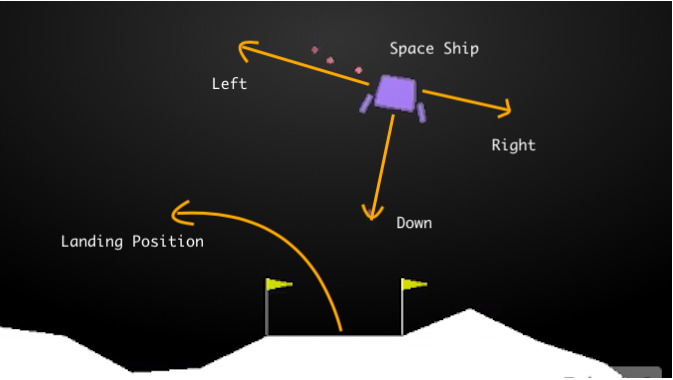
\includegraphics[width=\linewidth]{lander.png}
\caption{Lunar Lander in Opengym.}
\label{fig1}
\end{figure}

\section{Problem Statement}

The "Lunar Lander" problem consists of an 8-dimensional continuous state space $s$ and a discrete action space $a$, $(x, y, vx, vy, \theta, v\theta, leg_L, leg_R)$. $x$ and $y$ are the $x$ and $y$-coordinates of the lunar lander's position. $vx$ and $vy$ are the lunar lander's velocity components on the $x$ and $y$ axes. $\theta$ is the angle of the lunar lander. $\theta$ is the angular velocity of the lander. $leg_L$ and $leg_R$ are binary values to indicate whether the left leg or right leg of the lunar lander is touching the ground. So the states are six dimensional continuous state space with the addition of two more discrete variables. The four discrete actions available are: do nothing, fire the left orientation engine, fire the main engine, fire the right orientation engine.

The landing pad is always at coordinates (0,0). Coordinates consist of the first two numbers in the state vector. The total reward for moving from the top of the screen to the landing pad ranges from 100 - 140 points varying on the lander placement on the pad. If the lander moves away from the landing pad it is penalized the amount of reward that would be gained by moving towards the pad. An episode finishes if the lander crashes or comes to rest, receiving an additional -100 or +100 points respectively. Each leg ground contact is worth +10 points. Firing the main engine incurs a -0.3 point penalty for each occurrence. Landing outside of the landing pad is possible. Fuel is infinite, 

Problem in this project is how to let an agent learn to land the lunar ground on its first attempt. 

\section{Solution}

The problem is considered solved when the reward in one run achieving a score of 200 points or higher on average over 100 consecutive runs.

The agent is in a state $s$ and has to choose one action $a$, upon which it receives a reward $r$ and come to a new state $s{}'$, see equation (\ref{eqn:1}). The way the agent choosing actions is called $policy$. If the agent knows the expected reward of each action at every step, it will know exactly which action to perform at each step and finally learn the $policy$ that can achieve target.

All states that come in between an initial-state and a terminal-state is called one $episode$. The agent's goal it to maximize the total reward it receives during an episode. 

\begin{equation}\label{eqn:1}
    s \xrightarrow[]{\text{a}} r, s{}'
\end{equation}

Deep Q learning is the solution for this project. Deep Q learning uses neural network based on Q learning. In this report, Q learning (Section~\ref{sub:Q}) will be introduced first to facilitate the understanding of deep Q learning in (Section~\ref{sub:DQ}).

\begin{algorithm*}\label{al:1}
\SetAlgoLined
Initialize replay memory $D$ to a FIFO queue of capacity $N$\;
Initialize neural network training batch size $BS$\;
Initialize action-value function $Q$ with random weights\;
Construct neural network mapping from states to rewards\;
\For{$\text{episode}$ = 1, $M$}{
    Reset game environment\;
    Reward = 0 \;
    \For{$\text{step}$ = 1, STEP}{
    	Select an action $a$\;
    	\ \ \ \ Select a random action with probability $\epsilon$\;
    	\ \ \ \ Otherwise select $a$ = $\text{argmax}_a'$Q(s,$a'$)\;
    	Store $<s,a,r,s'>$ in replay memory $D$ after apply action $a$\;
    	Reward = Reward + r\;
    	s = $s'$\;
    	\If{replay memory buffer size $<=$ N and replay memory buffer size $>=$ BS and in every 3 episode}{
    	    Collect train batch randomly from replay memory\;
    		Train neural network using $(r-Q(s,a))^2$ as loss function and \;
    	}
    	\If{Done}{
    		Break
    	}
    }
    $\epsilon$ = $\epsilon$ * decay\;
    \If{$\text{Last 200 episodes rewards average} > 200$}{
    	Break
    }
 }
 \caption{Deep Q-learning}
\end{algorithm*}

\begin{figure*}
\begin{equation}\label{eqn:4}
\bigtriangledown _{\theta_i}L_i(\theta_i)=\text{E}_{s,a\sim \rho(.);s^{'}\sim\epsilon}    \left [(r+\gamma\text{max}_{a{}'} \text{Q}(s',a';\theta_{i-1}) - \text(Q)(s,a;\theta_{i}))\bigtriangledown _{\theta_i}\text{Q}(s,a;\theta_i)  \right ]   
\end{equation}
\end{figure*}

\begin{figure}[ht]
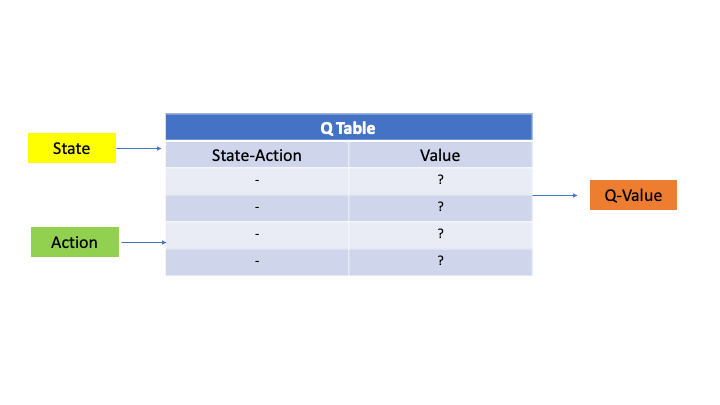
\includegraphics[width=\linewidth]{Q.png}
\caption{Q Learning.}
\label{fig7}
\end{figure}

\subsection{Q learning}\label{sub:Q}

In Q learning, the agent will perform the sequence of actions that will eventually generate the maximum total reward. 

\begin{figure}[ht]
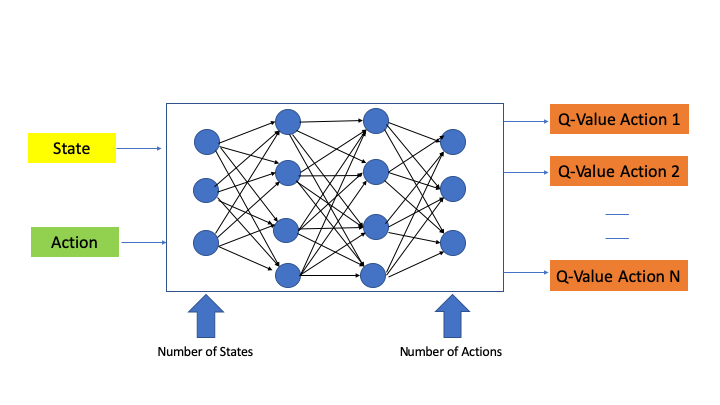
\includegraphics[width=\linewidth]{DeepQ.png}
\caption{Deep Q Learning.}
\label{fig8}
\end{figure} 

$Q(s,a)$ yielded from being at state $s$ and performing action $a$, is the immediate reward r(s,a) plus the highest Q-value possible from the next state $s'$, see in equation~(\ref{eqn:2}). $\gamma$ is a discount factor and $\gamma < 1$, it makes sure that the sum in the formula is finite. The lower the discount factor is, the less important future rewards are, and the agent will tend to focus on actions on immediate rewards only. $Q(s',a)$ recursively depends on $Q(s{}'',a)$, see equation~(\ref{eqn:3}). 

\begin{equation}\label{eqn:2}
    Q(s,a) = r(s,a) + \gamma \text{max}_a Q(s',a)
\end{equation}

\begin{equation}\label{eqn:3}
    Q(s,a) \rightarrow \gamma Q(s',a) + \gamma^2 Q(s'',a)......+\gamma^n Q(s^{''...n},a)
\end{equation}

The agent constantly performs the action that is believed to achieve the highest expected reward. The agent needs to try many different actions in many different states in order to try and learn all available possibilities and find the $policy$ which will maximize its overall reward, this is known as exploration, as the agent explores the environment. However, the agent should also use the informationit learned. The agent need to exploit and explore its knowledge to maximize the rewards it receives. Greedy policy, $\epsilon$-Greedy Policy allows agent to randomly explore. A number $\epsilon$ in the range of [0,1] is selected, if that number is larger than $\epsilon$, the greedy action is selected while a random action is selected if the number is lower. If $\epsilon$ = 0, the policy becomes the greedy policy, and if $\epsilon$ = 1, always explore. Such value iteration algorithm converge to the optimal action value function, $Q_i \rightarrow Q{}*$ as $i \rightarrow \infty$.  Finally, a Q table will be built for states to choose expected best action from, see Fig.\ref{fig7}.

\subsection{Deep Q Learning}\label{sub:DQ}

The continues states and descrete actions in 'Lunar Lander' OpenAI Gym scenario, require deep reinforcement learning~\cite{b1} to avoid the complexity of store Q table. Instead, the Q values are calculated by neural network by states and corresponding action rewards, see in Fig.\ref{fig8}.

The algorithm can be described in algorithm~\ref{al:1}. As reinforcement learning tasks have no pre-generated training sets which they can learn from, the agent must keep records of batches of the state-transitions it encountered in the replay memory buffer so it can learn from them later.

A function approximator is used to estimate the action-value function in deep Q learning, $Q(s,a;\theta) \approx Q^{*}(s,a)$. In the continuous agent state and discrete actions environment, a neural network function approximator with weights $\theta$ constructs a Q network. A Q network can be trained by minimising a sequence of loss functions $L_i(\theta_i)$ that changes at each iteration $i$,

\begin{equation}\label{eqn:5}
    L_i(\theta_i) = E_{s,a\sim\rho(.)}[(y_i - Q(s,a;\theta_i))^2]
\end{equation}

where $y_i = E_{s{}'\sim\epsilon}[r+\gamma \text{max}_{a{}'}Q(s{}',a{}',\theta_{i-1})|s,a]$ is the target for iteration $i$ and $\rho(s,a)$ is a probability distribution over sequences $s$ and action $a$ which is called behaviour distribution. Differentiating the loss function with respect to the weights.

Equation~(\ref{eqn:5}) is computationally expedient to optimise the loss function by stochastic gradient descent. The learning agent is following the Q learning algorithms~\cite{b3} with the neural network's assistance.

The deep Q learning is described in Algorithm I~(\ref{al:1}). Each step of batch experience is potentially used in many weight updates. Considering strong correlations between samples, randomizing the samples can break correlations and reduces the variance of the updates. When learning on-policy the current parameters determine the next data sample that the parameters are trained on. The timing for update of weights is also considered. Many experiments have been done to test the optimal number of episodes for updating the weights. The setting of batch size and the number of every other episodes to update weights are crucial parameters for rewards to converge. After several rounds of experiments, if weights update every N episode, N < 5, the network might not be stable and will not achieve rewards 200 or even drop below 0. And if the batch size is set too large or too small, the rewards also cannot converge.

Based on the theory of deep Q learning, the training result of 'Lunar Lander' is shown in Section~\ref{sec:result}.

\section{Result}\label{sec:result}

Neural network in the experiments is designed to be three layers, input layer, hidden layer and output layer. Batch size of neural network training data is set to be 64, the number of episodes that update neural network weights is set to be 5.

In the training, neural network is built with Keras~\cite{b4}. First, rewards at each training episode are demostrated in section~\ref{sec:rewards}. Then, hyperparameters differences' impact on the training is discussed in section~\ref{sec:hyper}. Results will be also simulated in section~\ref{sec:network} while neural network adopts various structures.

\subsection{Rewards}\label{sec:rewards}

In this subsection, the neural network has input layer with the number of neurons equaling to the number of states and relu activation function, first hidden layer with 512 neurons and relu activation function, second hidden layer with 256 neurons and relu activation, output layer with the number of naurons equaling to the number of actions and linear activation function. 

\begin{figure}[ht]
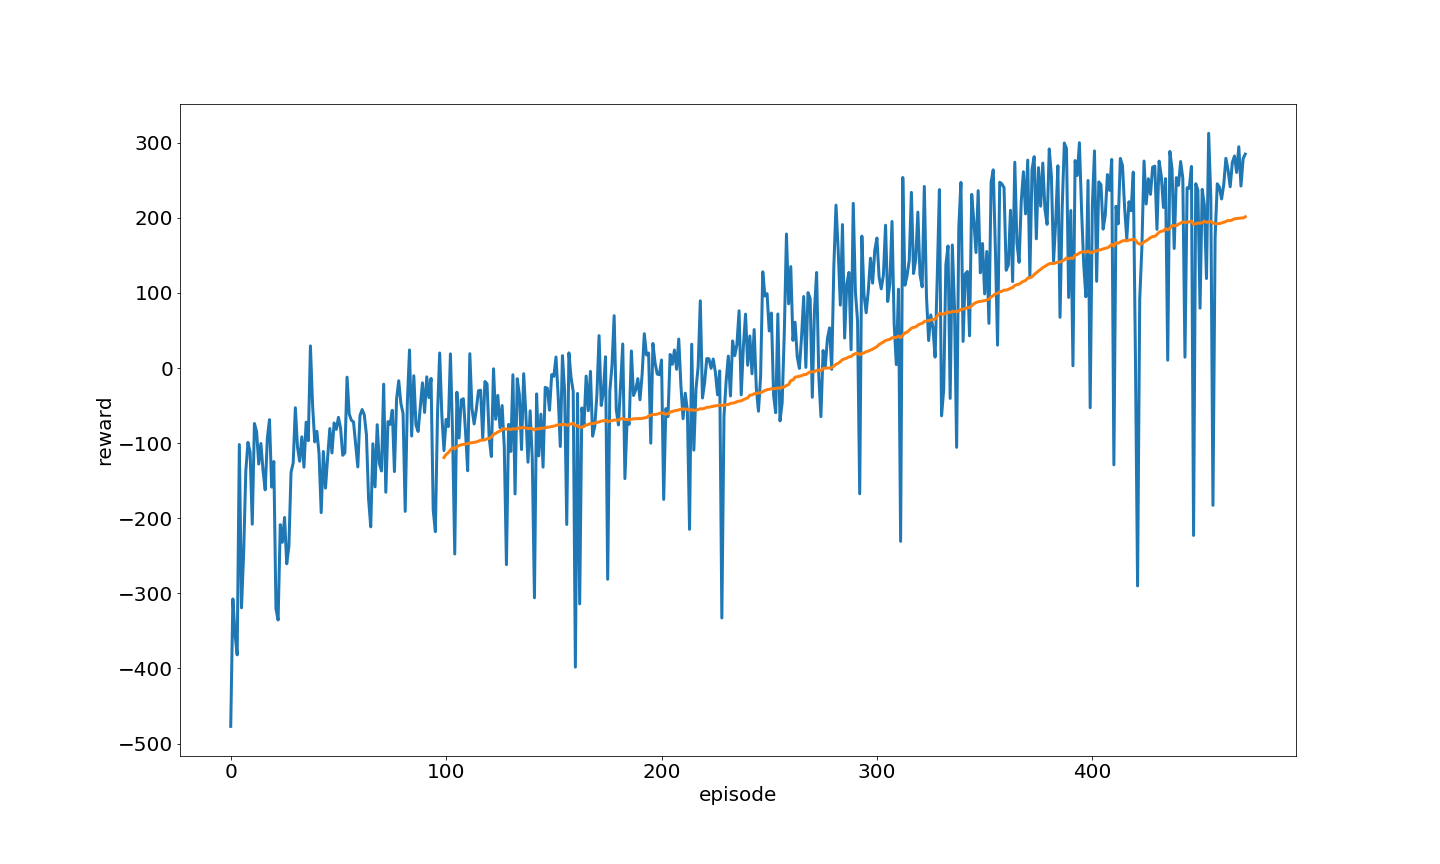
\includegraphics[width=\linewidth]{training_episode_reward.png}
\caption{Reward per episode for 8-512-256-4 linear activation layers}
\label{fig9}
\end{figure}

The parameters for this experiment is set as: learning rate = 0.001, $\epsilon = 1.0$, decay of $\epsilon= 0.995$, $\gamma$ = 0.99, the maximum number of training episodes is set to be 1000.

As seen in Fig~\ref{fig9}, the rewards are gradually increasing from about -477 to above 200. And when the number of training episode achieves 470, the average reward of recent 100 episodes converges to above 200, which achieve the success landing definition in the 'Lunar Landing' project. Then the agent based on deep Q learning is considered to be trained successfully.

\begin{figure}[ht]
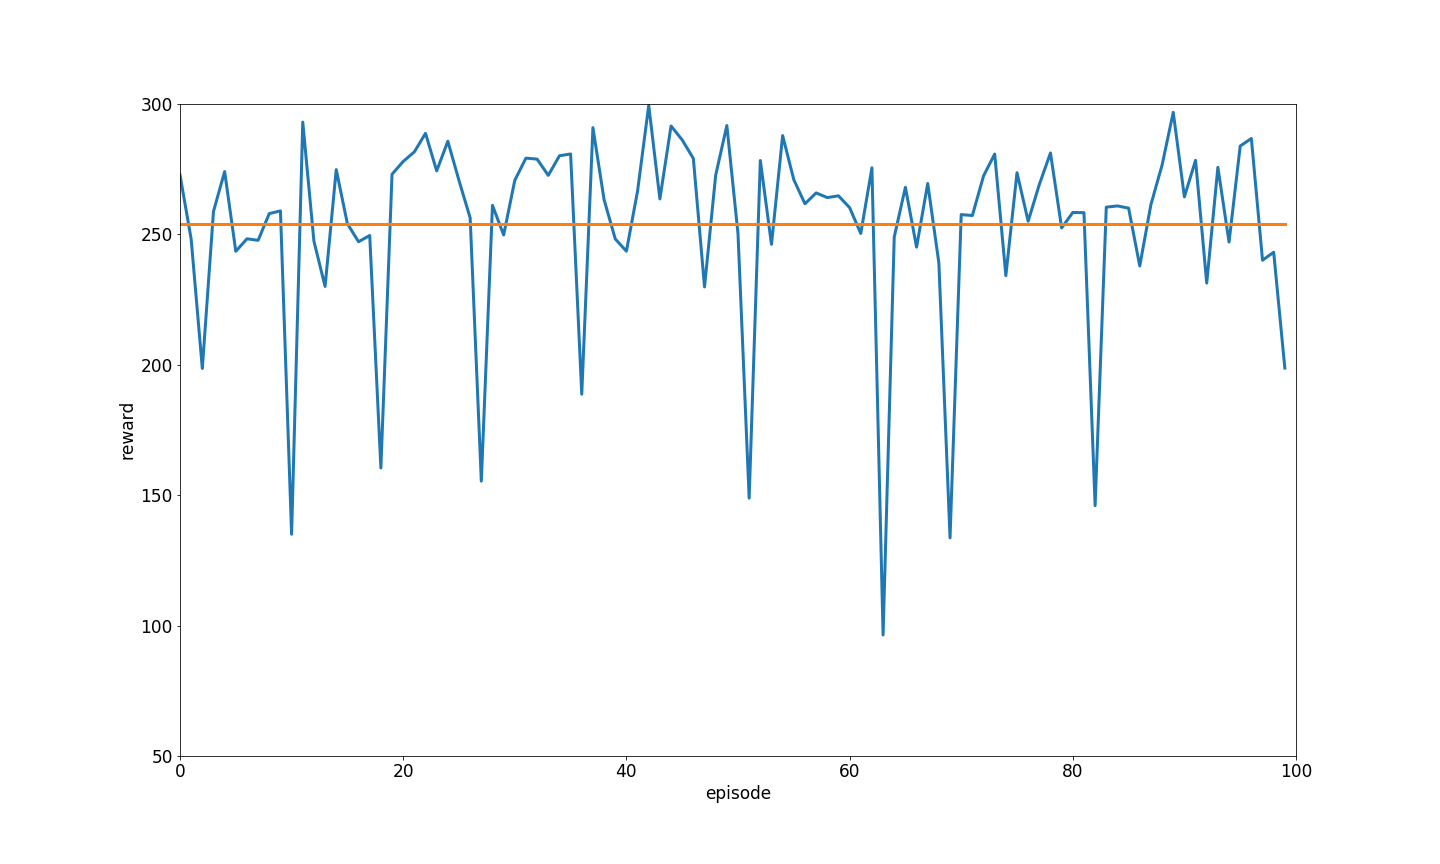
\includegraphics[width=\linewidth]{testing_episode_reward.png}
\caption{Reward per episode for 100 consecutive episodes using trained agent.}
\label{fig10}
\end{figure}

Next the trained agent is tested in complete different 100 consecutive randomly generalized scenarios of 'Lunar Landing', the rewards versus episode is plotted in Fig.~\ref{fig10}. The mean of 100 episode test rewards is 253.7. Among 100 episode, 90 episode rewards are larger than 200. The minimum episode reward is 96.37.

\subsection{Hyperparameters}\label{sec:hyper}

Hyperparameters like neural network learning rate, future Q value discount factor $\gamma$ and $\epsilon$ decay value will be discussed in this part.

\subsubsection{Neural network learning rate}\label{sec:lr}
Neural network learning rate is a hyperparameter that controls how much to change the model in response to the estimated error each round the model weights $\theta$ are updated. Too small learning rate may result in a long trainign process. Too large learning rate may result in a sub-optimal set of weights or an unstable training process. 

\begin{figure}[htbp]
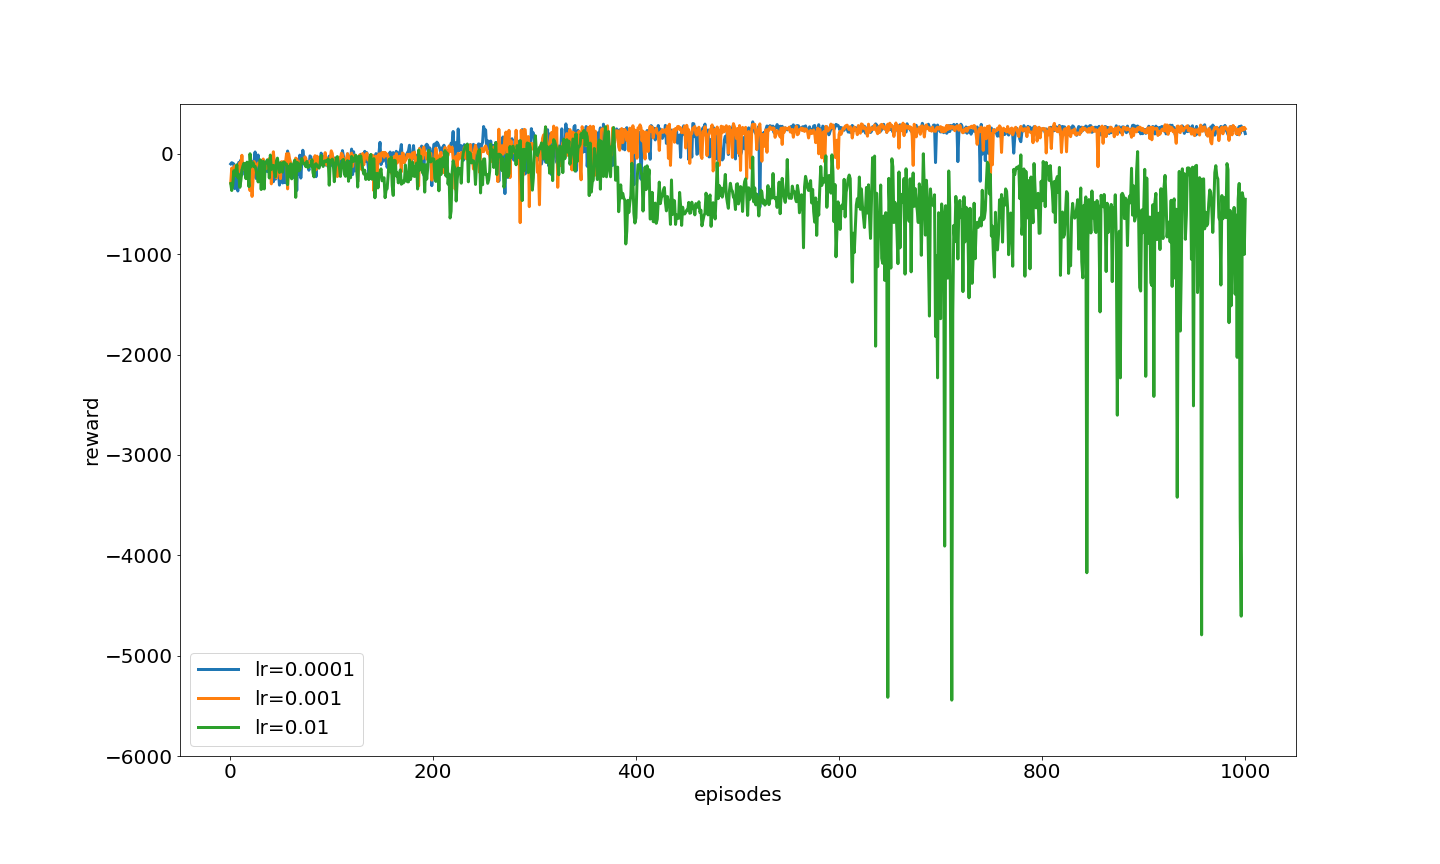
\includegraphics[width=\linewidth]{lr.png}
\caption{Reward per episode for different learning rates.}
\label{fig11}
\end{figure}

The parameters for this experiment is set as: learning rate ranges in [0.0001, 0.001, 0.01], $\epsilon = 1.0$, decay of $\epsilon= 0.995$, $\gamma$ = 0.99, the maximum number of training episodes is set to be 1000.

The results can be seen in Fig~\ref{fig11}. When learning rate is 0.0001, the average rewards of 1000 episode is 129.78, 53.4\% of episode rewards are larger than 200. The training process begins to converge at 479th episode. When learning rate is 0.001, the average rewards of 1000 episode is 122.68, 51.5\% of episode rewards are larger than 200. The training process begins to converge at 510th episode. When learning rate is 0.01, the average rewards of 1000 episode is -422.0, 0.9\% of episode rewards are larger than 200. The training process doesn't converge. 

\subsubsection{Discount factor $\gamma$}\label{sec:gamma}

Discount factor $\gamma$ quantifies how much importance future rewards weighing. It is also handy to approximate the noise in future rewards.

In this experiment, parameters are set as: $\gamma$ ranges in [0.999, 0.99, 0.9], learning rate = 0.001, $\epsilon$ = 1.0, $\epsilon$ decay = 0.995, training episodes = 1000.

\begin{figure}[htbp]
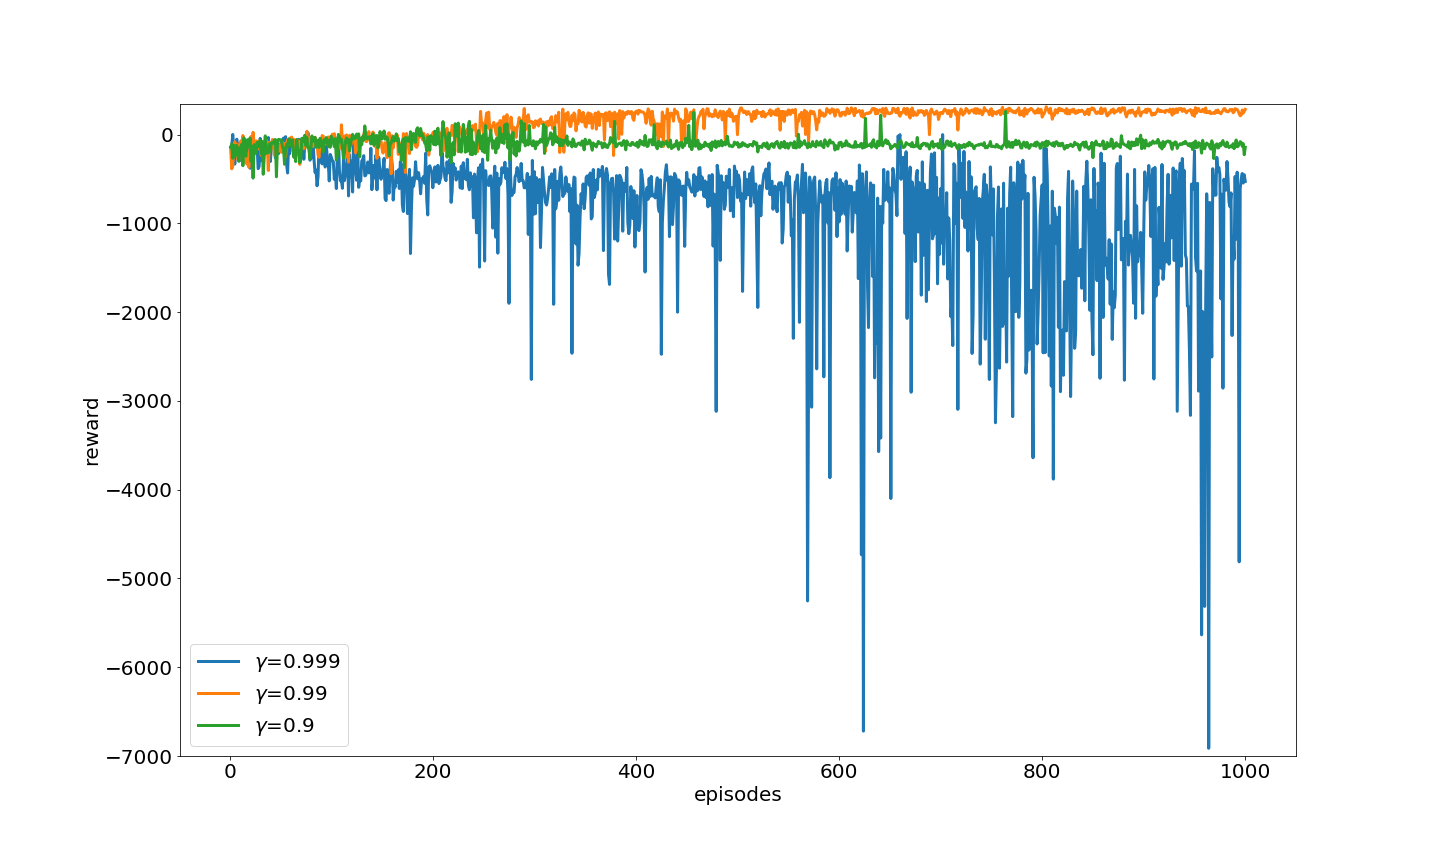
\includegraphics[width=\linewidth]{gamma.png}
\caption{Reward per episode for different $\gamma$ values.}
\label{fig12}
\end{figure}

It can be seen in Fig~\ref{fig12}. When $\gamma$ is 0.999, the average rewards of 1000 episode is -844.30, none episode rewards are larger than 200. When $\gamma$ is 0.99, the average rewards of 1000 episode is 146.70, 58.8\% of episode rewards are larger than 200. The training process begins to converge at 425th episode. When $\gamma$ is 0.9, the average rewards of 1000 episode is -101.84, 0.3\% of episode rewards are larger than 200. The training process doesn't converge. 

\subsubsection{$\epsilon$ decay}\label{sec:ed}

$\epsilon$ is associated with how random the agent take an action. As the learning goes on, $\epsilon$ should be decayed to stabilize and exploit the learned policy which converges to an optimal one, so that higher Q-values can be found in higher probability.

In this experiment, parameters are set as: $\epsilon$ decay ranges in [0.999, 0.995, 0.990], neural network learning rate = 0.001, $\epsilon$ = 1.0, $\gamma$ = 0.99, training episodes = 1000.

\begin{figure}[htbp]
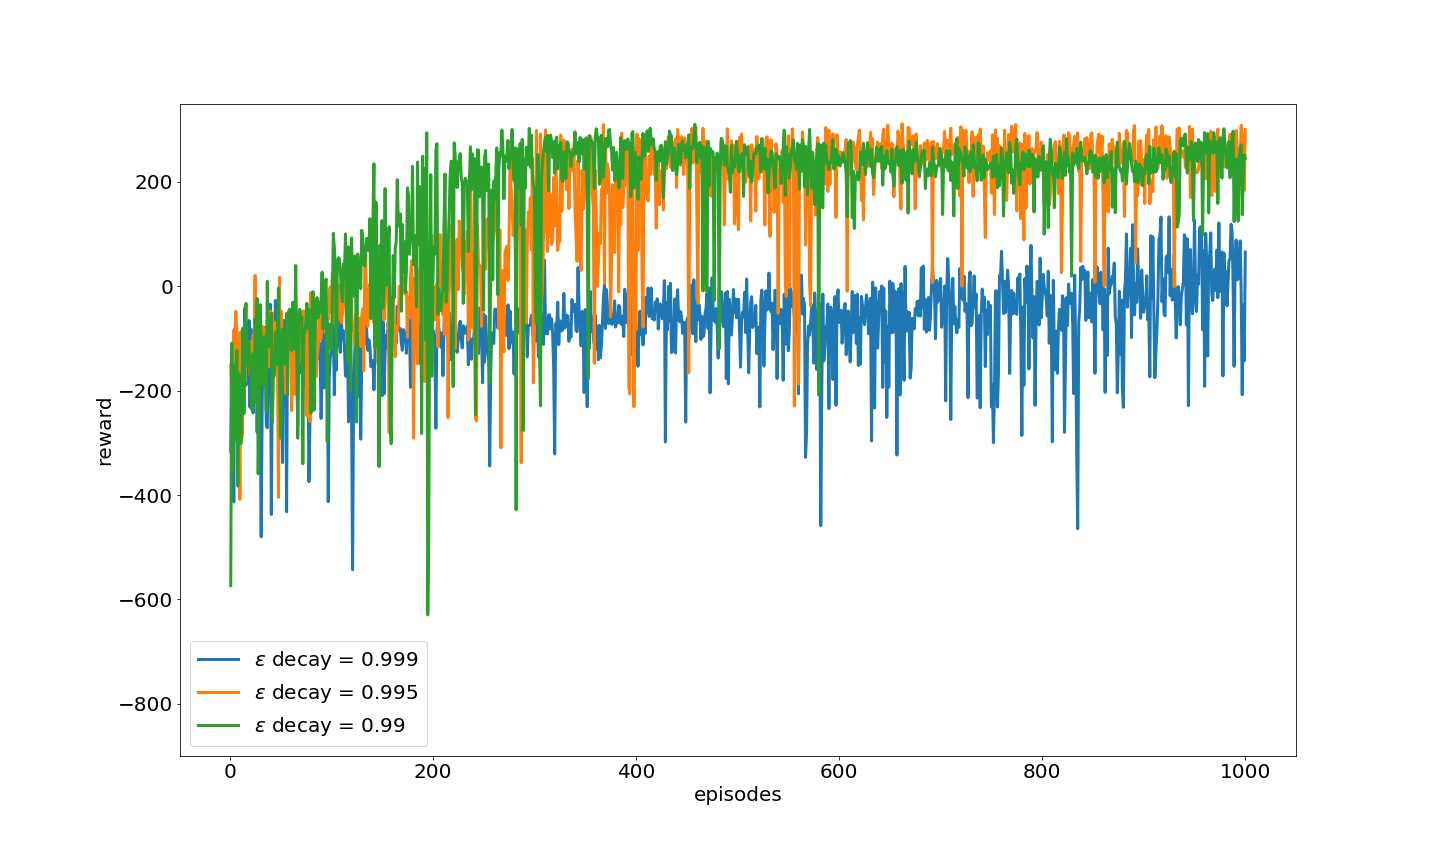
\includegraphics[width=\linewidth]{ed.png}
\caption{Reward per episode for different decay values.}
\label{fig13}
\end{figure}

The results can be seen in Fig~\ref{fig13}. When decay is 0.999, the average rewards of 1000 episode is -74.14, no episode rewards are larger than 200. When decay is 0.995, the average rewards of 1000 episode is 143.31, 55\% of episode rewards are larger than 200. The training process begins to converge at 378th episode. When decay is 0.99, the average rewards of 1000 episode is 170.69, 68.7\% of episode rewards are larger than 200. The training process rewards converges to 200 at episode 243. 

\subsection{Neural network structure}\label{sec:network}

Extra experiments have been done to explore the performance of different neural network architectures.

\subsubsection{Neural network setting 1: Simpler Setting}\label{sec:simple}

In this subsection, the neural network has a simpler setting: input layer with the number of neurons equaling to the number of states and relu activation function, first hidden layer with 128 neurons and relu activation function, second hidden layer with 64 neurons and relu activation, output layer with the number of neurons equaling to the number of actions and linear activation function.

\begin{figure}[htbp]
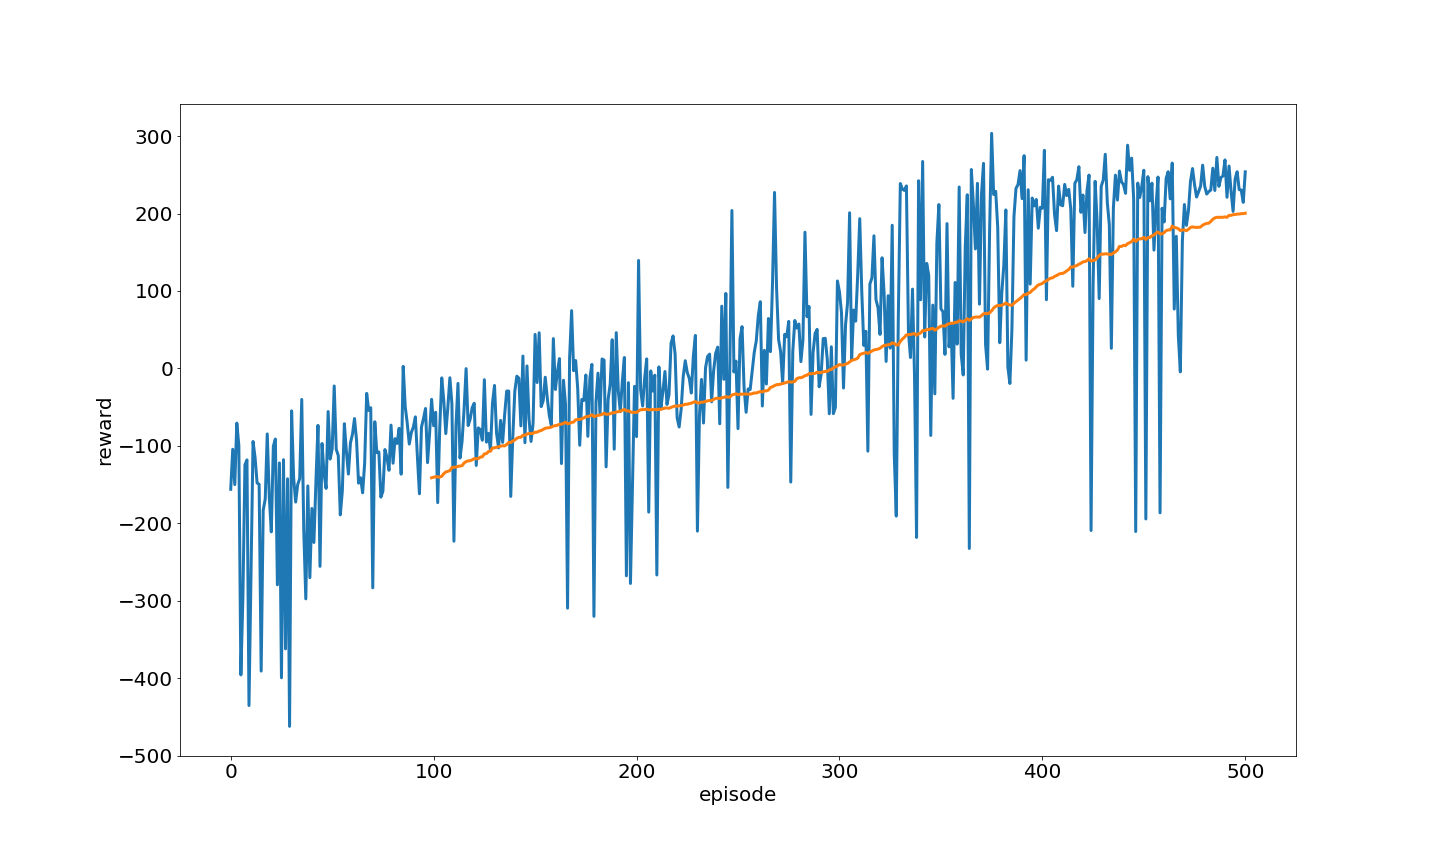
\includegraphics[width=\linewidth]{train_simple.png}
\caption{Reward per episode for 8-128-64-4 linear activation layers.}
\label{fig14}
\end{figure}

The training results are shown in Fig~\ref{fig14}, the rewards can converge to 200 in episode 500. 

\subsubsection{Neural network setting 2: Dropout Effect}\label{sec:dropout}

In this subsection, an experiment has been done to observe the dropout layer effect on the neural network. The other network layer settings are the same as subsection~\ref{sec:result}, besides an additional dropout layers with dropout rate of 0.2 is added before the output layer. Dropout is remarkably effective regularization method to reduce overfitting and improve generalization error in deep neural networks.

As can be seen in Fig~\ref{fig17}, the rewards do not converge in 1000 episodes. That means in the network contructed in subsection~\ref{sec:result}, there is no need to do dropout regularization.

\begin{figure}[ht]
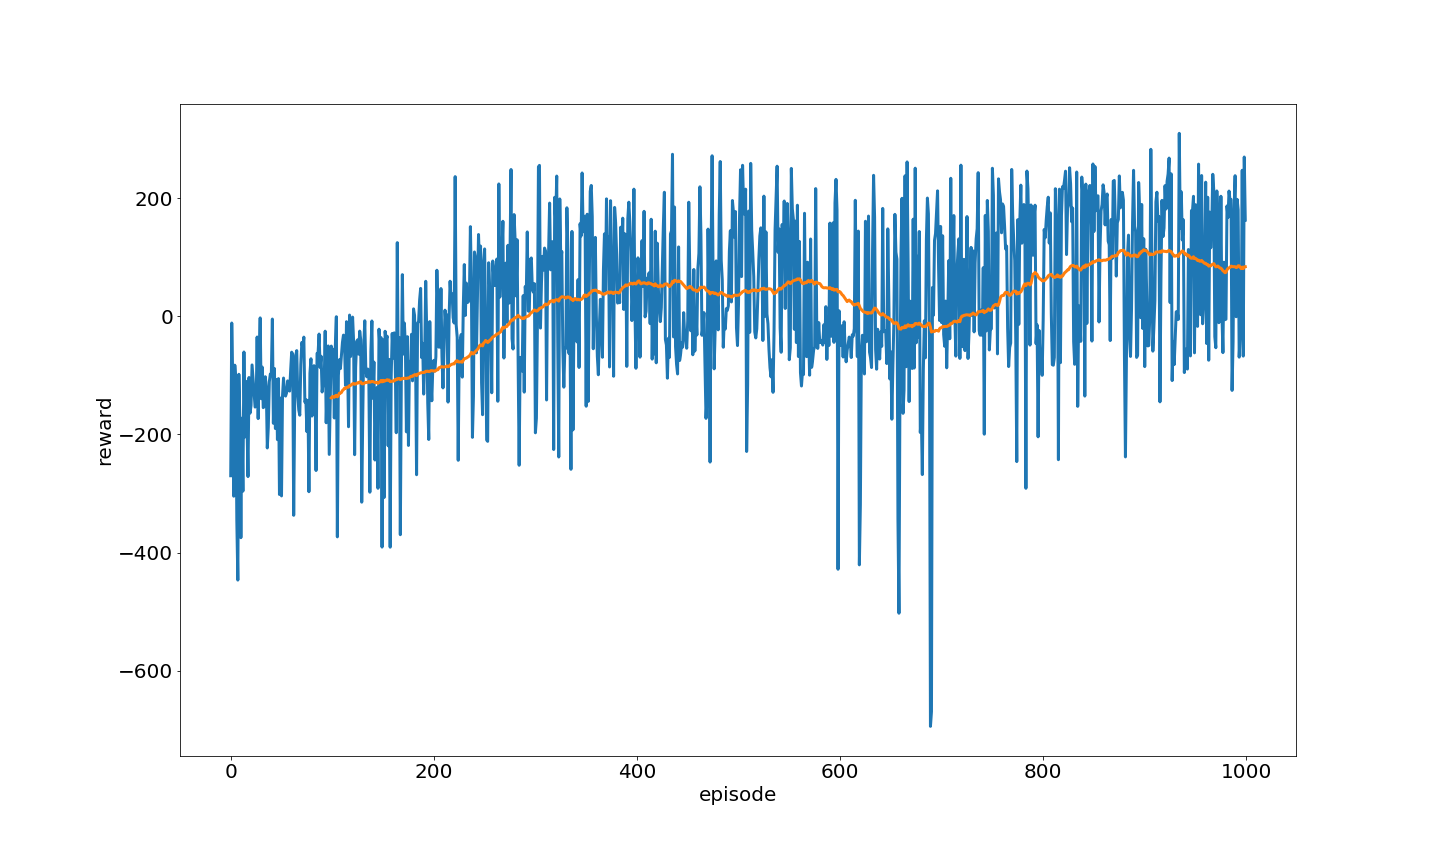
\includegraphics[width=\linewidth]{train_dropout.png}
\caption{Reward per episode for 8-512-256-4 linear activation layers with dropout 0.2.}
\label{fig17}
\end{figure}

\subsubsection{Neural network setting 3: Activation Setting}\label{sec:softmax}

In this subsection, the neural network adopts softmax activation instead of linear in the output layer. 

The neural network configurations are input layer with the number of neurons equaling to the number of states and relu activation function, hidden layers with 512, 256 neurons, output layer with the number of neurons equaling to the number of actions and softmax activation function.

It can be seen in Fig~\ref{fig15}, the rewards line cannot converge to 200 and even worse till -1067.73 in 500 episodes. That means the agent does not learn anything from the past experiences and environment using softmax activation.

\begin{figure}[htbp]
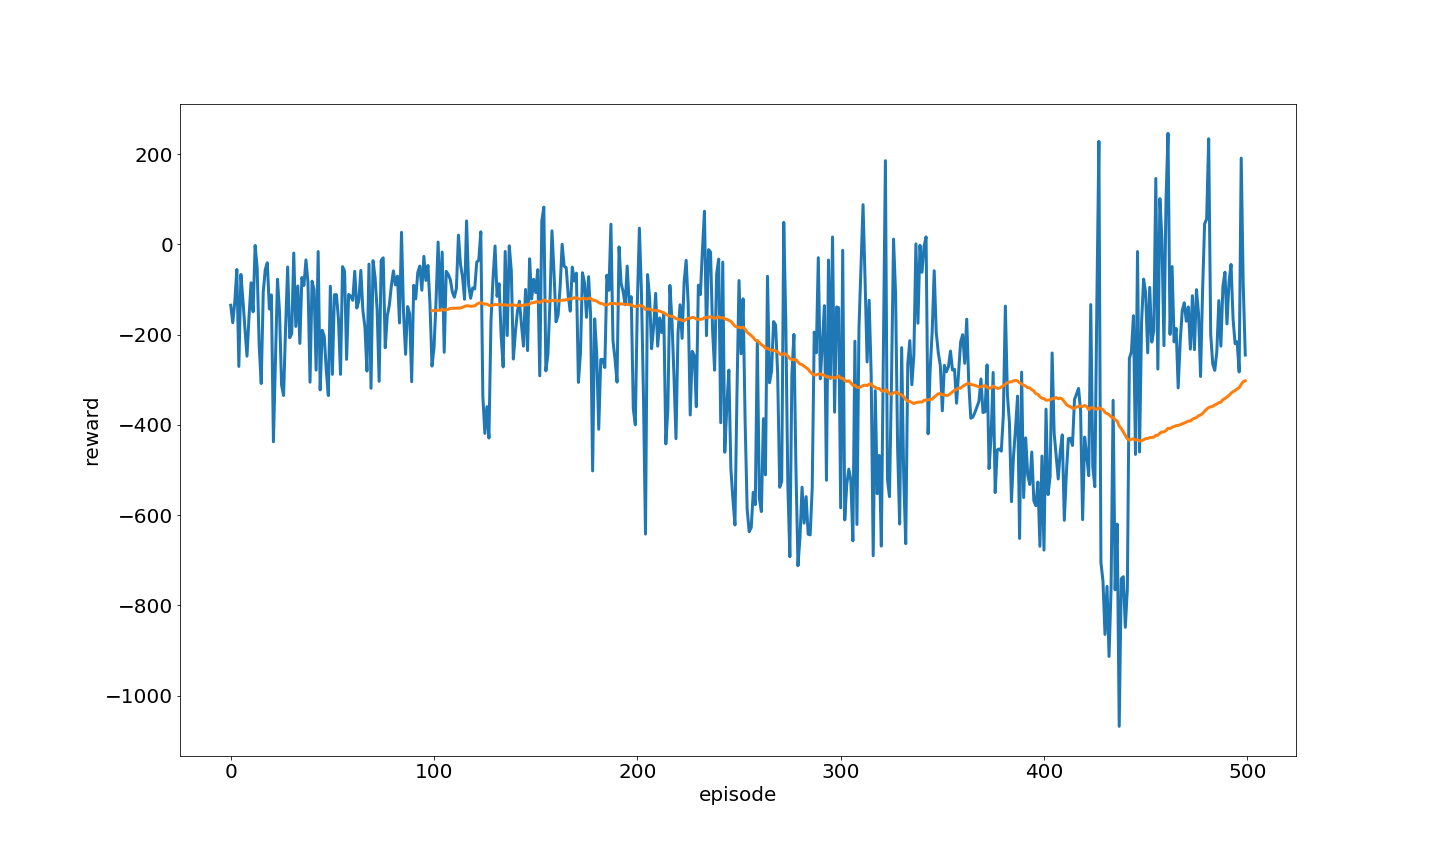
\includegraphics[width=\linewidth]{train_softmax.png}
\caption{Reward per episode for 8-512-256-4 softmax activation layers.}
\label{fig15}
\end{figure}

\section{Related work}
Currently, there are several works, that have noticed the dropback of the neural network training batch evenly randomly selection from replay memory buffer. There are kinds of training data selection algorithms, which consist of keeping training over its new behavior~\cite{b5} or conditioning each agent's value function on a fingerprint that disambiguates the age of the data sampled from the replay memory~\cite{b6}. Advanced designs of deep RL techniques lead to even lesser number of episodes for agent to learn the environment.

\section{Conclusion}
In this project, 'Lunar Lander' problem in OpenAI Gym is solved by deep reinforcement learning. Multiple experiments have been done to explore the effect to the learning process caused by different hyberparameters and different neural network desgins. 

\begin{thebibliography}{00}
\bibitem{b1} Volodymyr Mnih and Koray Kavukcuoglu and David Silver and Alex Graves and Ioannis Antonoglou and Daan Wierstra and Martin A. Riedmiller, \textit{Playing Atari with Deep Reinforcement Learning},CoRR abs/1312.5602, 322(10):891–921.
\bibitem{b2} Gym, https://gym.openai.com/
\bibitem{b3} Christopher JCH Watkins and Peter Dayan., Q-learning, \textit{Machine Learning}, 8(3-4):279-292, 1992
\bibitem{b4} Keras, https://keras.io/
\bibitem{b5} Tom Schaul, John Quan, Ioannis Antonoglou, David Silver, Prioritized Experience Replay, \textit{arXiv:1511.05952v4}, 2016
\bibitem{b6} Jakob Foerster, Nantas Nardelli, Gregory Farquhar, Triantafyllos Afouras, Philip H. S. Torr, Pushmeet Kohli, Shimon Whiteson, Stabilising experience replay for deep multi-agent reinforcement learning, \textit{ICML'17: Proceedings of the 34th International Conference on Machine Learning}, vol 70, Pages 1146–1155
\end{thebibliography}
\vspace{12pt}

\end{document}
